\section{Метод игнорирования пропусков}

    Посмотрим, как себя покажет метод <<игнорированя пропусков>> в случае пропусков, зависящих от данных. Для этого
    сначала теоретически исследуем свойство несмещенности и асимптотической несмещенности оценки, 
    полученной по этому методу, в случае цензурирования. Также исследуем зависимость смещения оценки от порога
    цензурирования $c$.

    Смещение будем искать по определению:
    \begin{equation*}
        b(n, \theta_0, c) = E_{\theta_0}\{\hat{a}\} - \mu,
    \end{equation*}
    где $\theta_0$ --- истинное значение параметра распределения, $\mu$ --- матожидание $x_i$.
    Также обозначим за $p_\xi(x, \theta)$ плотность распределения элементов выборки. получим
    \begin{equation*}
        b(n, \theta_0, c) = \int_{\Rb^n}T(X)\pvec(X,\theta_0)\dd X - \mu,
    \end{equation*}
    где
    \begin{equation*}
        \pvec(X,\theta) = \prod_{i=1}^{n}p_\xi(x_i,\theta).
    \end{equation*}
    В случае цензурирования вид статистики $T(X)$ будет зависеть от значений выборки, поэтому
    представим пространство $\Rb^n$ как сумму областей
    \begin{equation*}
        A_\alpha = \{X \in \Rb^n\,:\,x_i > c \Leftrightarrow i \in \alpha\}, \quad \alpha \subseteq \{1,\ldots,n\}.
    \end{equation*}
    Тогда по свойствам интеграла
    \begin{equation*}
        E_{\theta_0}\{\hat{a}\} = \sum_\alpha \int_{A_\alpha}T(X)\pvec(X,\theta_0)\dd X.
    \end{equation*}
    Рассмотрим $A_\varnothing = \{X \in \Rb^n\,:\,x_1 \le c,\ldots,x_n \le c\}$. В ней статистика имеет вид
    \begin{gather*}
        T(X) = \frac1n \sum_{i=1}^{n}x_i, \\
        \begin{aligned}
            &\int_{A_\varnothing}T(X)\pvec(X,\theta_0)\dd X = \frac1n\sum_{i=1}^{n}\int_{A_\varnothing}x_i\pvec(X,\theta_0)\dd X =\\
            &= \frac1n\sum_{i=1}^{n}\int_{-\infty}^{c}p_\xi(x_1,\theta_0)\dd x_1\int_{-\infty}^{c}\cdots\int_{-\infty}^{c}x_i p_\xi(x_i,\theta_0)\dd x_i\int_{-\infty}^{c}\cdots\int_{-\infty}^{c}p(x_n,\theta_0)\dd x_n =\\
            &= \int_{-\infty}^{c}xp(x,\theta_0)\dd x \cdot \bigg(\int_{-\infty}^{c}p(x,\theta_0)\dd x\bigg)^{n-1}.
        \end{aligned}
    \end{gather*}
    Теппрь рассмотрим $A_i = \{X \in \Rb^n\,:\,x_1\le c,\ldots,x_{i-1}\}$, где статистика принимает вид
    \begin{equation*}
        T(X) = \frac{x_1+\ldots+x_{i-1}+x_{i+1}+\ldots+x_n}{n-1}, \\
    \end{equation*}
    и рассуждая аналогично, получаем
    \begin{equation*}
        \int_{A_i}T(X)\pvec(X,\theta_0)\dd X = \\\int_{-\infty}^{c}\!\!xp(x,\theta_0)\dd x \cdot \bigg(\int_{c}^{+\infty}\!\!p(x,\theta_0)\dd x\bigg) \bigg(\int_{-\infty}^{c}\!\!p(x,\theta_0)\dd x\bigg)^{n-2}
    \end{equation*}
    Проведя такие же преобразования, получим общую формулу для $A_\alpha$:
    \begin{equation*}
        \int_{A_\alpha}T(X)\pvec(X,\theta_0)\dd X = \\\int_{-\infty}^{c}\!\!xp(x,\theta_0)\dd x\,\bigg(\!\!\int_{c}^{+\infty}\!\!p(x,\theta_0)\dd x\bigg)^{|\alpha|} \bigg(\!\!\int_{-\infty}^{c}\!\!p(x,\theta_0)\dd x\bigg)^{n-1-|\alpha|}
    \end{equation*}
    Примем $T(X) = 0$ при $X \in A_{\{1,\ldots,n\}}$, обозначим интегралы для краткости
    \begin{equation*}
        a = \int_{-\infty}^{c}x p_\xi(x,\theta_0)\dd x, \quad b = \int_{-\infty}^{c}p_\xi(x,\theta_0)\dd x
    \end{equation*}
    и получим
    \begin{align*}
        E_{\theta_0}\{\hat{a}\} &= \sum_{i=0}^{n-1}a C_n^i b^{n-1-i}(1-b)^i = ab^{n-1}\sum_{i=0}^{n-1}C_n^i\left(\frac{1-b}{b}\right)^i = \\
        &= ab^{n-1}\left(\left(\frac{1-b}{b}+1\right)^n - \left(\frac{1-b}{b}\right)^n\right) = \frac{a}{b}(1-(1-b)^n).
    \end{align*}
    Учитывая, что $0 < b < 1$, 
    \begin{equation*}
        \lim_{n\to +\infty}\frac{a}{b}(1-(1-b)^n) = \frac{a}{b} = \frac{\int_{-\infty}^{c}x p_\xi(x,\theta_0)\dd x}{\int_{-\infty}^{c}p_\xi(x,\theta_0)\dd x}
    \end{equation*}
    Для примера возьмем экспоненциальное распределение с параметром $\lambda_0$. Получим
    \begin{equation*}
        \lim_{n\to +\infty}b(n,\lambda_0,c) = \lim_{n\to +\infty}\frac{\int_{0}^{c}x \lambda_0 e^{-\lambda_0 x}\dd x}{\int_{0}^{c}\lambda_0 e^{-\lambda_0 x}\dd x} - \frac{1}{\lambda_0} = -\frac{c}{1-e^{c\lambda_0}}
    \end{equation*}
    Эта функция стремится к 0 по модулю при $c\to +\infty$, но никогда не равна нулю, следовательно наша оценка будет смещенной для всех $c$ и $\lambda$.

    Теперь получим оценки по методу <<игнорирования пропусков>> в компьютерном эксперименте. Создадим выборку с гауссовским распределением с параметрами $a = 1$ и $\sigma^2 = 2$. Затем смоделируем 4 ситуации 
    пропусков данных:
    \begin{enumerate}
        \item Без пропусков
        \item Случайные пропуски, $m(x) = 0.5$
        \item Полное цензурирование, $c = 1.5$
        \item Частичное цензурирование, случай $m(x) = \left\{
                                                        \begin{array}{ll}
                                                            0.5, & x \geq 1.5 \\
                                                            0, & x < 1.5
                                                        \end{array}\right.$.
    \end{enumerate}
    Теперь удалим пропуски из выборки и будем вести дальнейшую работу с полученной выборкой размером $T' \leq T$. Будем рассчитывать оценку 
    матожидания вида
    \begin{equation*}
        \hat{a} = \frac{1}{T'}\sum_{i=1}^{T'}x_i .
    \end{equation*}

    На рисунках 1 и 2 показаны сами оценки и их вариация соответственно для различных размеров выборки $T$ и для четырех ситуаций 
    с пропусками данных.

    \begin{figure}[ht]
        \subcaptionbox*{Рисунок 1}[.49\linewidth]{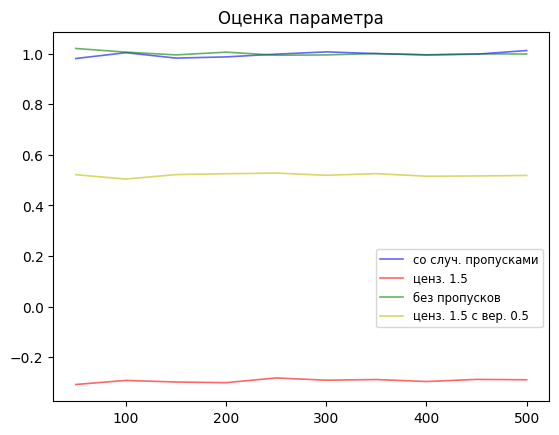
\includegraphics[width=\linewidth]{pict1.png}}
        \hfill
        \subcaptionbox*{Рисунок 2}[.49\linewidth]{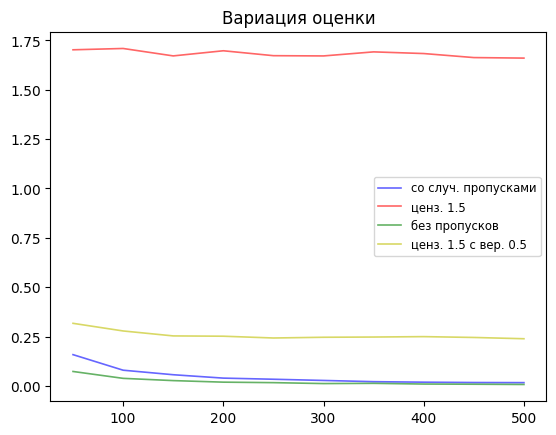
\includegraphics[width=\linewidth]{pict2.png}}
    \end{figure}